\documentclass[a4paper,12pt]{memoir}
\usepackage{msiu_term_work}

\lstset{language=Ruby,inputencoding=utf8/koi8-r,basicstyle=\small,
stringstyle=\ttfamily,xleftmargin=1cm}

\begin{document}
\renewcommand{\contentsname}{{\Large{Содержание}\hfill}}

\title{Методы хранения и обработки информации}
{Вычисление значений выражений, содержащих только записанные в 
десятичной системе счисления натуральные числа, абсолютная величина 
которых не превосходит $3999$. Вычисление мощности множества точек 
пересечения границы выпуклой оболочки с замкнутым единичным кругом 
с центром в начале координат. Нахождение суммы длин проекций полностью 
невидимых рёбер полиэдра, центр которых находится на расстоянии строго 
меньше единицы от плоскости $x=2$}
{141131}
{Д.\+А.~Хотелов}
{к.ф.-м.н., доцент}
{Е.\+А.~Роганов}
{2015}

\section{Введение}
В данной курсовой работе рассматриваются модификации трёх эталонных про-
ектов «Стековый копилятор формул», «Выпуклая оболочка» и 
«Изображение проекции полиэдра», реализованных на объектно-ориентированном 
языке программирования высокого уровня Ruby.

Проект «Стековый копилятор формул»\cite{compf} представляет собой 
программную реализацию некоторой функции $\tau$, действующей из 
множества цепочек одного языка $L_1$ (в рассматриваемом случае 
это язык арифметических формул) в множество цепочек 
другого $L_2$ (язык программ стекового калькулятора) таким образом, 
что $\forall\omega\;\in\;L_1$ семантика 
цепочек $\omega$ и $\tau(\omega)\;\in\;L_2$ совпадает. 
Говоря другими словами, компилятор реализует перевод 
с одного языка на другой с сохранением смысла.

Проект «Выпуклая оболочка»\cite{convex} решает задачу индуктивного 
перевычисления выпуклой оболочки последовательно поступающих точек плоскости 
и таких её характеристик, как периметр и площадь.

Проект «Изображение проекции полиэдра»\cite{polyedr} выполняет построение изображения 
полиэдра с учётом удаления невидимых линий.

Целями работы являются:
\begin{itemize}
\item Проект «Стековый копилятор формул» требуется модифицировать так, 
чтобы вычислялись значения выражений, содержащих только записанные в 
десятичной системе счисления натуральные числа, абсолютная величина 
которых не превосходит 3999.
\item В проект «Выпуклая оболочка» добавить вычисление мощности 
множества точек пересечения границы выпуклой оболочки 
с замкнутым единичным кругом с центром в начале координат.
\item Модифицировать проект «Изображение проекции полиэдра» таким образом, 
чтобы определялась и печаталась следующая характеристика полиэдра: 
сумма длин проекций полностью невидимых рёбер, центр которых находится 
на расстоянии строго меньше единицы от плоскости $x=2$.
\end{itemize}

Для того чтобы выполнить полученные задания, необходимо было изучить 
особенности языка Ruby, подробно разобрать каждый эталонный проект и 
применить полученные знания в области информатики, 
компьютерной математики и аналитической геометрии на плоскости и 
в пространстве.

\section{Модификация проекта «Стековый копилятор формул»}
\subsection{Постановка задачи}

Модифицируйте эталонный проект таким образом, чтобы вычислялись 
значения выражений, содержащих только записанные в десятичной системе 
счисления натуральные числа, абсолютная величина которых 
не превосходит 3999. Результат должен быть выдан 
в десятичной системе счисления.

После запуска файла \verb|calc.rb| пользователю предлагается ввести 
арифметическое выражение, затем происходит вывод результата 
вычисленного выражения. Допустим для выражения $45*2-10$ должен 
выводиться ответ \verb|80|. В эталонном проекте можно вводить 
лишь цифры от $0$ до $9$.

\subsection{Решение задачи и модификация кода}

Чтобы выполнить поставленную задачу, необходимо знать где 
обрабатывается каждый символ и как 
обработать число: $10 < n < 5000$.

Обработка каждого символа осуществляется в файле \verb|compf.rb| 
в методе \verb|compile| класса \verb|Compf|. Необходимо уметь 
обрабатывать символ, длина которого больше одного. Кроме этого следует 
учитывать проверку каждого символа в файле \verb|calc.rb| 
в методе \verb|check_symbol| класса \verb|Calc|. Здесь модификация 
наиболее проста: необходимо допускать длину цифр больше $1$ и 
не допускать значения самих цифр больше $3999$. Эта проверка 
реализована следующим образом:
\begin{small}
\verbatiminput{programms/check.rb}
\end{small}

Сама идея обработки символов заключается в том, чтобы перед обработкой 
очередного символа увеличивать длину цепочки на число(если это число), 
пока не встретится любой другой символ. Затем обрабатывается 
последовательность этих чисел, а именно преобразование из 
строкого представления в числовое и добавление этого числа в стек 
для подсчёта итогового результата, и затем обрабрабатывается только 
что прибывший символ. Реализация метода \verb|compile| 
класса \verb|Compf|:
\begin{small}
\verbatiminput{programms/compile.rb}
\end{small}

Пример работы данной реализации(рис.~\ref{fig:example_calc}):
\begin{figure}[ht!]
\begin{center}
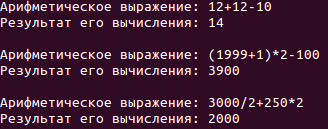
\includegraphics[scale=0.6]{images/example_calc}
\end{center}
\vspace*{-8mm}
\caption{}\label{fig:example_calc}
\end{figure}

\section{Модификация проекта «Выпуклая оболочка»}
\subsection{Постановка задачи}

Модифицируйте эталонный проект таким образом, чтобы вычислялась мощность 
множества точек пересечения границы выпуклой оболочки 
с замкнутым единичным кругом с центром в начале координат.

После запуска программа предлагает пользователю ввести последовательно 
координаты вершин выпуклой оболочки. Введённая точка индуктивно 
добавляется в выпуклую оболочку. Нам же необходимо вместе со 
значениями периметра и площади выпуклой оболочки выводить мощность 
множества точек пересечения границы выпуклой оболочки 
с замкнутым единичным кругом с центром в начале координат.

Допустим для точек $A(-1,-1)$, $B(1,1)$ и $C(1,-1)$ программа выдаст 
в качестве ответа \verb|infinity|, потому что отрезок $AB$ 
пересекает единичный круг в бесконечном множестве точек, но при 
добавлении точки $D(-1,1)$ множество перевычисляется, и в качестве ответа 
выдаётся \verb|4|, потому что квадрат $ABCD$ описывает окружность и 
пересекается с ней в четырёх точках.

\subsection{Решение и модификация кода}

Для решения данной задачи нам необходимо находить расстояние от центра 
круга до стороны выпуклой оболочки. Это задание сводится к нахождения 
расстояния от точки до отрезка(точка нам задана $O(0,0)$, а отрезком 
является сторона выпуклой оболочки).

Допустим нам дан отрезок $AB$ и точка $O$. Расстоянием от точки $O$ 
до отрезка $AB$ является отрезок $OA$, $OB$ или высота из точки $O$ 
до $AB$(если эта высота падает на $AB$). Высота падает 
на $AB$, если $\angle OAB$ и $\angle OBA$ являются острыми или 
один из них прямой, другой острый. Нам даны лишь координаты этих точек. 
С помощью метода \verb|dist| класса \verb|R2Point| можно найти 
расстояние всех трёх сторон. Затем по теореме косинусов находим 
$\cos\angle A$ и $\cos\angle B$:
$$OB^2 = AO^2+AB^2-2\cdot AO\cdot AB\cos\angle A \Rightarrow 
\cos\angle A = \frac{AO^2+AB^2-OB^2}{2\cdot AO\cdot AB}$$

Аналогично находим $\cos\angle B$. Затем определяем -- является 
ли угол острым или прямым. Если выполняется условие: 
$0 \leqslant \cos\alpha \leqslant 1$, то угол острый или прямой. 
Саму высоту мы находим из площади треугольника: $S=\frac12\cdot 
AB\cdot h \Rightarrow h=\frac{2\cdot S}{AB}$. Сторона $AB$ известна, 
площадь можно найти с помощью метода \verb|R2Point.area| 
класса \verb|R2Point|.

Теперь можно найти растояние от точки до стороны выпуклой оболочки, 
как наименьшее значение длины среди сторон $AO$, $OB$ и $h$.

\newpage

После этого можно найти множество точек пересечения отрезка с 
замкнутым единичным кругом в начале координат. Если расстояние меньше 
единицы, то множеством точек пересечения будет являться 
\verb|infinity|(рис.~\ref{fig:ro_0}):
\begin{figure}[ht!]
\begin{center}
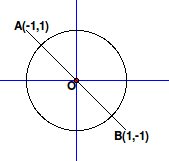
\includegraphics[scale=0.6]{images/ro_0}
\end{center}
\vspace*{-8mm}
\caption{}\label{fig:ro_0}
\end{figure}

Если расстояние равно единицы, то множеством точек пересечения будет 
являться \verb|1|(рис.~\ref{fig:ro_1}):
\begin{figure}[ht!]
\begin{center}
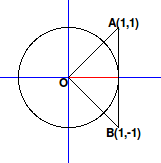
\includegraphics[scale=0.6]{images/ro_1}
\end{center}
\vspace*{-8mm}
\caption{}\label{fig:ro_1}
\end{figure}

Если расстояние больше единицы, то множеством точек пересечения будет 
являться \verb|0|(рис.~\ref{fig:ro_more}):
\begin{figure}[ht!]
\begin{center}
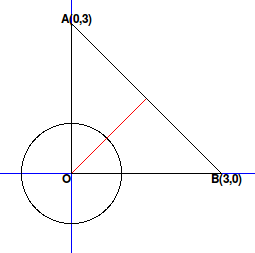
\includegraphics[scale=0.45]{images/ro_more}
\end{center}
\vspace*{-8mm}
\caption{}\label{fig:ro_more}
\end{figure}

Метод \verb|R2Point.intersect|, который принимает две точки в качестве 
аргумента и выдаёт множество точек пересечения этого отрезка с 
единичным кругом описан в классе \verb|R2Point| и реализован 
следующим образом:
\begin{small}
\verbatiminput{programms/multi.rb}
\end{small}

Теперь можно находить множество точек пересечения стороны выпуклой 
оболочки с кругом. Рассмотрим это вычисление для всей выпуклой оболочки.

Если выпуклой оболочкой является точка, то множество точек 
пересечения с кругом будет сама эта точка, либо множество будет 
равняться нулю. Для отрезка мы уже знаем как найти это множество, 
а многоугольник рассмотрим подробно.

Так как ответом пересечения стороны выпуклой оболочки и круга 
может быть число или \verb|infinity|, то целесообразно хранить сумму 
этих чисел(\verb|@n_point|), количество 
\verb|infinity|(\verb|@n_infinity|) и итоговый ответ(\verb|@n_points|) 
в разных переменных. Для того, чтобы менять значения этих переменных 
в зависимости от удаления или добавления ребра выпуклой оболочки, 
написан метод \verb|oper_with_n_p|, принимающий на вход две точки для 
отрезка и ещё один аргумент, позволяющий обрабатывать ситуацию, когда 
ребро выпуклой оболочки удаляется или добавляется. Этот метод 
находится в секции \verb|private| для того, чтобы он был виден 
только в классе \verb|Polygon|. Листинг данного метода:
\begin{small}
\verbatiminput{programms/oper.rb}
\end{small}

Теперь с помощью этого метода можно индуктивно вычислять множество 
точек пересечения замкнутого круга с центром в начале координат.

При добавлении новой точки необходимо учитывать удаление освещенных 
рёбер, соответственно мощность множества точек пересечения необходимо 
пересчитывать. Чтобы сделать это индуктивно, мы используем дек, в 
который помещаем значение точек -- вершин выпуклой оболочки.

Сам процесс индуктивного перевычсления мощности множества точек 
пересечнения можно представить в таблице(табл.~\ref{tab:tab1}), которая приведена ниже:
\begin{table}[h!]
\begin{tabular}{|p{6cm}|p{10cm}|}
\hline
Удаляем ребро, соединяю-
щее начало и конец дека,
если оно освещено нашей
точкой:
&
\verb|oper_with_n_p(@points.last,@points.first,"del")|\\
\hline
Удаляем освещенные реб-
ра из начала дека:
&
\verb|oper_with_n_p(p, @points.first, "del")|\\
\hline
Удаляем освещенные реб-
ра из конца дека:
&
\verb|oper_with_n_p(p, @points.last, "del")|\\
\hline
Обрабатываем два добавленных ребра:
&
\verb|oper_with_n_p(t, @points.first)|
\verb|oper_with_n_p(t, @points.last)|\\
\hline
\end{tabular}
\caption{}\label{tab:tab1}
\end{table}

Пример работы программы представлен на рис.~\ref{fig:ex1}. 
Добавляются точки ABC и результат: \verb|infinity|. Затем добавляется 
точка D(рис.~\ref{fig:ex2}), множество точек пересчитывается и 
результатом будет число $4$ -- четыре точки пересечения выпуклой 
оболочки с кругом.
\begin{figure}[ht!]
\begin{center}
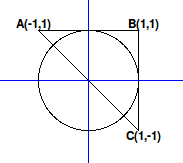
\includegraphics[scale=0.6]{images/circ}
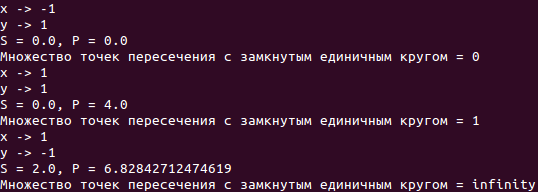
\includegraphics[scale=0.5]{images/ex1}
\end{center}
\vspace*{-8mm}
\caption{}\label{fig:ex1}
\end{figure}

\begin{figure}[ht!]
\begin{center}
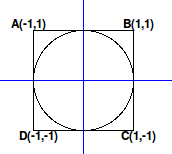
\includegraphics[scale=0.6]{images/circ2}
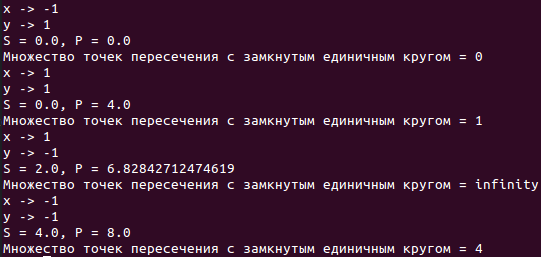
\includegraphics[scale=0.4]{images/ex2}
\end{center}
\vspace*{-8mm}
\caption{}\label{fig:ex2}
\end{figure}

\section{Модификация проекта «Изображение проекции полиэдра»}
\subsection{Постановка задачи}

Модифицируйте эталонный проект таким образом, чтобы определялась и печаталась следующая характеристика полиэдра: сумма длин проекций полностью невидимых рёбер, центр которых находится на расстоянии строго меньше $1$ от плоскости $x=2$.

При выполнении задания должна использоваться следующая трактовка величин,
задающих полиэдр в geom - файле: реальные координаты вершин полиэдра вычисляются с учетом вращений пространства, задаваемых углами Эйлера, и коэффициента
гомотетии.

Ребро будем называть полностью невидимым, если оно полностью затемнено и нет ни одного отрезка в переменной \verb|@gaps| класса \verb|Edge|. В переменной \verb|@gaps| хранятся только незатемнённые отрезки от грани.

\subsection{Решение задачи}
Для решения поставленной задачи нам необходимо находить длину проекции невидимого ребра. Так как ребро задаётся двумя точками в пространстве, то проекциями этих точек на плоскость $XY$ будут соответственные точки с координатами $(x;y)$ без учёта z-координаты. Поэтому длину ребра находим через две точки $A(x_1;y_1)$ и $B(x_2;y_2)$ по формуле:
$$l=\sqrt{(x_2-x_1)^2+(y_2-y_1)^2}$$

Так же нам необходим центр ребра, но здесь надо учитывать то, что нам нужна лишь x-координата, потому что мы определяем расстояние от этого центра до плоскости $x=2$. Для этого нам достаточно найти центр ребра только по x-координате. Нужный центр ребра вычисляем по формуле:
$$\frac{(x_1+x_2)}{2}$$

Остаётся определить условие того, что центр ребра находится на расстоянии строго меньше единицы от плоскости $x=2$. Центр ребра должен быть больше единицы, но меньше трёх.

\subsection{Модификация кода}

Метод \verb|some_len|, который находит длину полностью невидимого ребра, центр которого находится на расстоянии строго меньше единицы от плоскости $x=2$, мы определили в файле \verb|shadow/polyedr.rb| в классе \verb|Edge|. Листинг данного метода:
\newpage
\begin{small}
\verbatiminput{programms/some_len.rb}
\end{small}

Но нам нужна сумма всех таких рёбер полиэдра. Для этого мы определили метод \verb|some_sum_len_edges| в классе \verb|Polyedr|. В данном методе мы обходим все рёбра и складываем нужные нам с помощью метода \verb|some_len|. Листинг метода \verb|some_sum_len_edges|:
\begin{small}
\verbatiminput{programms/some_sum_len_edges.rb}
\end{small}

Затем остаётся лишь вывести эту сумму, но она должна выводиться после учёта затемнения рёбер. 

Данную сумму выводим в файле \verb|run_polyedr.rb|: \verb|puts poliedr.some_sum_len_edges|.

Пример работы данной реализации представлен на рис.~\ref{fig:king}(Для наглядности нарисуем плоскости $x=1$ и $x=3$, а также центры рёбер, попадающие строго в этот диапазон):
\begin{figure}[ht!]
\begin{center}
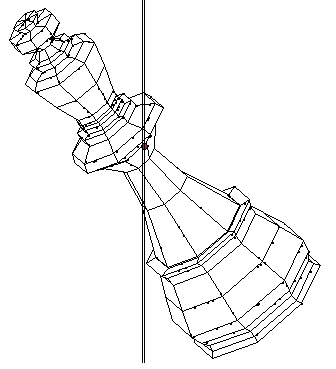
\includegraphics[scale=0.3]{images/king}
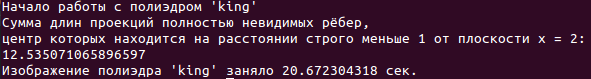
\includegraphics[scale=0.5]{images/king_ex}
\end{center}
\vspace*{-8mm}
\caption{}\label{fig:king}
\end{figure}

\begin{thebibliography}{}

\bibitem{compf}
\link{http://edu1.msiu.ru/f/7275-material\_ici\_toc.zip/index.html}~---
Описание проекта «Стековый копилятор формул».

\bibitem{convex}
\link{http://edu1.msiu.ru/f/7561-material\_ici\_toc.zip/index.html},
\link{http://edu1.msiu.ru/f/7591-material\_ici\_toc.zip/index.html}~---
Описание проекта «Выпуклая оболочка».

\bibitem{polyedr}
\link{http://edu1.msiu.ru/f/7780-material\_ici\_toc.zip/index.html},
\link{http://edu1.msiu.ru/f/7811-material\_ici\_toc.zip/index.html},
\link{http://edu1.msiu.ru/f/7863-material\_ici\_toc.zip/index.html}~---
Описание проекта «Изображение проекции полиэдра».

\bibitem{ruby}
\link{http://ru.wikipedia.org/wiki/Ruby}~---
Википедия (свободная энциклопедия) о языке Ruby.

\bibitem{rlatex}
С.М. Львовский.
{\em Набор и вёрстка в системе \LaTeX, 3-е изд., испр. и доп.}~---
М., МЦНМО, 2003. Доступны исходные тексты этой книги.

\bibitem{texbook}
D.~E.~Knuth. {\em The \TeX{}book.}~---
Addison-Wesley, 1984. Русский перевод:
Дональд~Е.~Кнут.
{\em Все про \TeX.}~--- Протвино, РД\TeX, 1993.

\end{thebibliography}

\newpage
\section{Приложение}
\subsection{Изменения, внесённые в эталонный проект «Выпуклая оболочка»}
Изменения в файле \verb|convex.rb|
\begin{tiny}
\verbatiminput{programms/pol.patch}
\end{tiny}

Изменения в файле \verb|r2point.rb|
\begin{tiny}
\verbatiminput{programms/r2.patch}
\end{tiny}

Изменения в файле \verb|tk_drawer.rb|
\begin{tiny}
\verbatiminput{programms/draw.patch}
\end{tiny}

Изменения в файле \verb|run_tkconvex.rb|
\begin{tiny}
\verbatiminput{programms/run.patch}
\end{tiny}

Изменения в файле \verb|convex_spec.rb|
\begin{tiny}
\verbatiminput{programms/convex_spec.patch}
\end{tiny}


\end{document}
